\chapter{Hadoop}\label{cap:hadoop}
\noindent This chapter tries to expose with simplicity the defining fundamentals of Hadoop architecture. Initially abstract concepts will be introduced to give way to more particular and deep ideas that explore Hadoop implementation of the MapReduce model in two layers: the processing and the storage subsystem.

\section{The Beginnings}\label{sec:origen}
\noindent Hadoop roots its origins in \emph{Apache Nutch}, Mike Cafarella and Doug Cutting's implementation of an open source web index and search engine. Nutch project began in 2002. In spite of the Internet being notoriously smaller at the time, Nutch's underlying technology was unable to make it scale to manage the billion pages that comprised the \emph{old} Internet. But in 2003 Google publishes a research paper introducing \emph{GFS} (\emph{Google File System}) \cite{gfs}, a file system to be used across their clusters of commodity pcs that greatly simplified its deployment. Nutch will inherit a large part of the concepts detailed there translated in their own distributed file system implementation (\emph{NDFS}).

Also in 2004 appeared another publication \cite{googlemapreduce} that presented MapReduce, bringing about successive efforts to port Nutch algorithms to adapt to the emerging model. In mid 2005 most of Nutch code run following MapReduce guidelines over NDFS.

Both NDFS and Nutch MapReduce implementation were generic enough to be used without refactoring beyond web page indexing. In 2006 an unrelated project was constituted to extend Nutch's potentially reusable parts to widen their applicability context. This project was called Hadoop. In 2008 \emph{Yahoo!} announced that the index for their search engine in production was being continually refreshed by 10,000 Hadoop nodes. This same year Hadoop is brought out to the world becoming an Apache-backed project corroborating its success.

Nowadays, Hadoop is without doubt the MapReduce implementation most widely used by a broad range of companies.

\section{General Hadoop Architecture}\label{sec:arquitecturahadoop}
\noindent Hadoop composition differentiates four modules:
\begin{description}
 \item[Hadoop Common:] A module containing the parts used across the implementation. It is mainly comprised of scripts and configuration tools.
 \item[Hadoop MapReduce:] The module implementing the MapReduce processing model.
 \item[Hadoop YARN:] A general purpose framework abstracted from Hadoop MapReduce. It is employed to manage resources and schedule executions in distributed environments.
 \item[Hadoop DFS:] The distributed file system sustaining inputs and outputs from Hadoop clusters.
\end{description}

Hadoop architecture corresponds to the \emph{Master-Worker} archetype where two roles on each cluster appear: a unique Master and various Workers. These roles, and thus responsibilities, are fixed to different nodes by the cluster admin. If necessary, e.g. for maintenance, the admin may freely re-set the roles to new cluster nodes, only requiring job resubmissions if the Master role were reassigned.

This section will almost exclusively center around MapReduce and Hadoop DFS (HDFS) modules to expose the functionally covered with Hadoop. Hadoop YARN, as discussed, is a subsystem resulting from the isolation of scheduling and processing, both found together in the old --- pre Hadoop 2 --- MapReduce module, retaining task distribution and planning within YARN. This way, YARN is allowed to untie from Hadoop allowing for deployments where YARN orchestrates an implementation-agnostic working set. As of this writing, Hadoop YARN is still an alpha version.

Figures \ref{fig:hadoopmapredhdfs} and \ref{fig:hadoopmapreddfs} exhibit a high level vision of Hadoop architecture. Figure \ref{fig:hadoopmapredhdfs} shows an hypothetical deployment with HDFS. Figure \ref{fig:hadoopmapreddfs} shows a particular Hadoop installation with another supporting distributed file system.

\begin{figure}[tbp]
\begin{center}
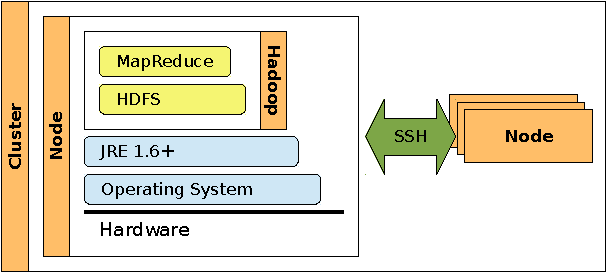
\includegraphics[width=0.7\textwidth]{imagenes/015.pdf}
 \caption{Hadoop over HDFS}
\label{fig:hadoopmapredhdfs}
\end{center}
\end{figure}

\begin{figure}[tbp]
\begin{center}
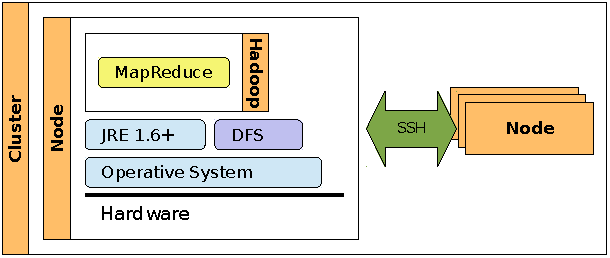
\includegraphics[width=0.7\textwidth]{imagenes/016.pdf}
 \caption{Hadoop over another DFS}
\label{fig:hadoopmapreddfs}
\end{center}
\end{figure}

From the figures it can be deduced that Hadoop runs atop a \emph{Java Virtual Machine} (emph{JVM}), that MapReduce requires a DFS implementation to rely on and that inter-node communication is conveyed through \emph{SSH} tunnels over TCP. Every module includes a web server (\emph{Jetty}) to ease collecting and reporting status information.

\section{Hadoop Distributed File System}\label{sec:hdfs}
\noindent HDFS has been designed to act as archival repository for huge masses of data whose main access pattern be \emph{write-one} \emph{read-many}. While it is no requisite for a data query to follow this access pattern, HDFS performance shines with read queries in batch mode. The underlying infrastructure, again, is composed by commodity pcs that HDFS manages to transform into a reliable, scalable, fault tolerant, self-balancing and network traffic reducing data store. Yet, as individual nodes are regular pcs, in HDFS converge some operating limitations:

\begin{itemize}
 \item High data access time. HDFS prioritizes large reads in batches and thus, reading small files is generally discouraged. As complement though, HDFS delivers \emph{very} high throughput by leveraging parallel reads on the cluster.
 \item High data writing time on many small files. Writing a file changes a block. Every file that be smaller than the HDFS block size must be persisted in a single block. That changed block must be send out across the network to keep the file system consistently updated. Thus, appending to many files requires updates in many blocks that would require synchronizing over the network.
 \item Multiple writes to the same file or ``\emph{not-append}'' operations are not supported. HDFS is not a \emph{POSIX}-compilant file system implementing only a set of operations to try to maximize data throughput in distributed environments.
\end{itemize}

To organize storage, HDFS takes from traditional operating systems the concept of block: an abstraction of the particular drive structure with a double purpose:

\begin{description}
 \item[Lowering DFS complexity:] Writing a block comprises storing data and meta-data, and handling information related to locate those data on disk. Using the block as the minimum organizational structure simplifies location expressions.
 \item[Incrementing flexibility:] files are free to grow over the size of an HDFS block.
\end{description}

To lay local drive blocks in position, HDFS makes use of two processes: the \emph{DataNode} and the \emph{NameNode}. Besides, as support, from Hadoop 0.21.0 onward it is permitted the optional deploying of a \emph{Backup Node} and a \emph{Checkpoint Node} in the same cluster.

\subsection{Node Roles}\label{subsec:rolesnodos}
\noindent Figure \ref{fig:desplieguehdfs} shows a layered down HDFS deployment. In dotted line appear both the Backup Node and the Checkpoint Node.

\begin{figure}[tbp]
\begin{center}
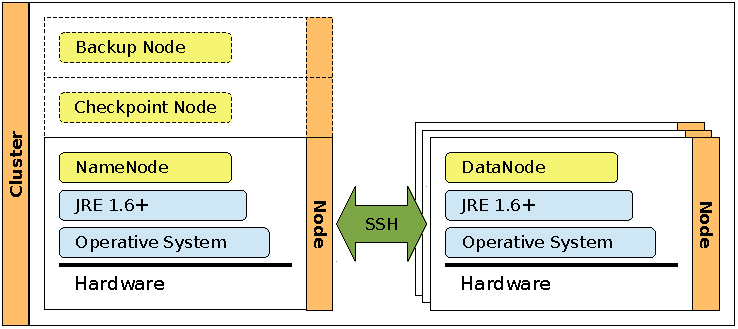
\includegraphics[width=0.85\textwidth]{imagenes/017.pdf}
 \caption{Typical HDFS deployment}
\label{fig:desplieguehdfs}
\end{center}
\end{figure}

\subsubsection{DataNode}\label{subsubsec:datanode}
\noindent DataNodes are those processes within nodes that handle the storage of HDFS blocks in their local drives. Every time a write to a file in a block succeeds, the DataNode in charge of the operation signals its supervising NameNode so that it could keep track the modifications to the DFS as they happen.

\subsubsection{NameNode}\label{subsubsec:namenode}
\noindent The NameNode is the process appointed to deal with the name space of the cluster. It has to handle the file system tree and meta-data that make possible recovering data from the DFS. It is such an important process that if it went down, every piece of data in HDFS would get lost, rendering impossible to match files with their container blocks. Therefore, the NameNode is seldom deployed with no Checkpoint Nodes or Backup Nodes in case the HDFS data were not stored elsewhere.

The information about the file system, meta-data, is persisted to the NameNode both in memory and disk. In this latter form, meta-data is managed in two files: one contains the name space of the file system as an image (\texttt{fsimage}), the other progressively appends the changes to the fsimage (\emph{edits}) as a log. When the DataNode starts, it compiles an fsimage afresh by merging the existing fsimage with the edits file. As soon as changes to the HDFS are reported from the NameNodes, the DataNode will update the edits log but without touching the fsimage. In a typical secured deployment, the edits file is kept in memory within the NameNode host computer, on the local file system and remotely via NFS.

\subsubsection{Checkpoint Node}\label{subsubsec:checkpointnode}
\noindent El fin que se persigue agregando un nodo de este tipo es mitigar los problemas relacionados con la ca\'ida de operaci\'on del NameNode. Peri\'odicamente, el Nodo de Checkpoint va generando puntos de restauraci\'on, o \emph{checkpoints}, siguiendo la misma estrategia que en el NameNode, es decir, usando \texttt{fsimage} y \texttt{edits}. Cada cierto tiempo, se descargar\'an ambos ficheros desde el NameNode y se fundir\'an, formando una nueva imagen actualizada que ser\'a transferida al NameNode. Cuando haya finalizado con \'exito la operaci\'on, el NameNode tendr\'a que purgar la imagen antigua e iniciar un nuevo fichero de log que albergue los cambios que se vayan sucediendo.


\subsubsection{Backup Node}\label{subsubsec:backupnode}
\noindent El Nodo de Backup provee la misma funcionalidad de generaci\'on de puntos de restauraci\'on que el Checkpoint Node pero usando una aproximaci\'on diferente. Para mantener sincronizado su espacio de nombres con el del NameNode que plagia, este tipo de nodo se descarga el \texttt{fsimage} al arrancarse y lo actualiza con las modificaciones que vaya captando el NameNode. Adicionalmente y cada cierto tiempo, el Backup Node actualiza su \texttt{fsimage} con los \texttt{edits}, creando un punto de restauraci\'on asociado.\newline

En comparaci\'on con el Checkpoint Node, este nodo consume menos ancho de banda de red ya que no necesita descargarse el \texttt{fsimage} y los \texttt{edits} del NameNode para mantener el sincronismo de estado.\newline

Como apuntes finales, destacar que de momento (versi\'on 1.0.4 de Hadoop), s\'olo se soporta un Nodo de Backup por NameNode o m\'ultiples Nodos de Checkpoint, y que la presencia de un Backup Node habilita la posibilidad de correr el NameNode sin almacenamiento persistente, delegando esa res\-pon\-sa\-bi\-li\-dad al Nodo de Backup.


\subsection{Topolog\'ia de red}\label{subsec:topologiared}
\noindent Una de las partes fundamentales de un sistema de ficheros en un entorno distribuido es proveer al usuario de un mecanismo transparente, que garantice la persistencia de la informaci\'on en \'el contenida manteniendo un cierto nivel de prestaciones. El HDFS utiliza una t\'ecnica, ya citada para los cloud, la replicaci\'on, que proporciona altas prestaciones, escalabilidad y tolerancia a fallo, al tiempo que limita la congesti\'on de red controlando la ubicaci\'on y el n\'umero de copias de los bloques en el centro de datos.

\subsubsection{Distancia entre nodos}\label{subsubsec:distnodos}
\noindent Para poder soportar las prestaciones comentadas, es fundamental que el NameNode, que es quien gestiona la distribuci\'on de las r\'eplicas de los bloques, tenga cierto conocimiento de la organizaci\'on f\'isica de los nodos que participan en el despliegue. La idea fundamental es tratar de mantener un equilibrio en la separaci\'on de las copias, entendida como la \emph{distancia f\'isica} entre los nodos que almacenan cada una: la distancia media entre r\'eplicas es proporcional tanto a la tolerancia a fallo del sistema, como al ancho de banda consumido para enviar cada r\'eplica. Recordemos que el ancho de banda de red disponible para transferir informaci\'on entre distintos nodos se reduce a medida que los alejamos, o visto de desde otro \'angulo, que la transferencia ser\'a m\'as costosa cuanto mayor sea la distancia entre el nodo que contenga el bloque original y aquel que vaya a albergar la r\'eplica. Es decir, ser\'ia id\'oneo, para equilibrar la separaci\'on entre r\'eplicas, definir una m\'etrica que calculase la distancia entre dos nodos cualesquiera.\newline

Como los nodos de las redes IP siguen una estructura de \'arbol invertido, y la red de un cl\'uster Hadoop es de este tipo, se podr\'ia considerar, como aproximaci\'on de la distancia f\'isica entre nodos, la \texttt{distancia internodal}: \emph{la suma de las distancias de los nodos al ancestro com\'un m\'as pr\'oximo}.\newline

Tal y como se ha comentado, HDFS utiliza RPC sobre TCP/IP a trav\'es de SSH para la comunicaci\'on entre nodos, lo cual (capa IP) no aporta informaci\'on de localizaci\'on \emph{concreta} de cada nodo dentro del despliegue. Para concretar la distancia internodal y as\'i poder hacer un reparto \'optimo de las copias, es necesario configurar HDFS para que cada IP sea mapeada a una posici\'on concreta, de tantas componentes ---\texttt{(centro de datos, rack, nodo)}, por ejemplo--- como niveles haya en la red. La figura \ref{fig:distnodos} muestra un ejemplo con los valores m\'as comunes de la distancia internodal. Veremos c\'omo se calcula para el caso \texttt{d=4}.\newline

Fij\'andonos en la figura \ref{fig:distnodos}, el bloque azul representa la copia original, y el bloque amarillo, destino del arco azul con etiqueta \texttt{d=4}, la r\'eplica. Ambos bloques se encuentran en nodos de distintos racks en el mismo centro de datos. El ancestro com\'un m\'as pr\'oximo entre ellos ser\'a el enrutador que maneje el tr\'afico entre ambos racks. Adem\'as, cada nodo tiene que atravesar otro enrutador de rack, otro ancestro m\'as pr\'oximo a los nodos, que dirige la paqueter\'ia dentro del rack. Con lo que tenemos \emph{dos pasos} (distancia 2) para llegar al router que conecta ambos racks por cada nodo; sumando ambas distancias obtenemos el resultado.

\begin{figure}[tbp]
\begin{center}
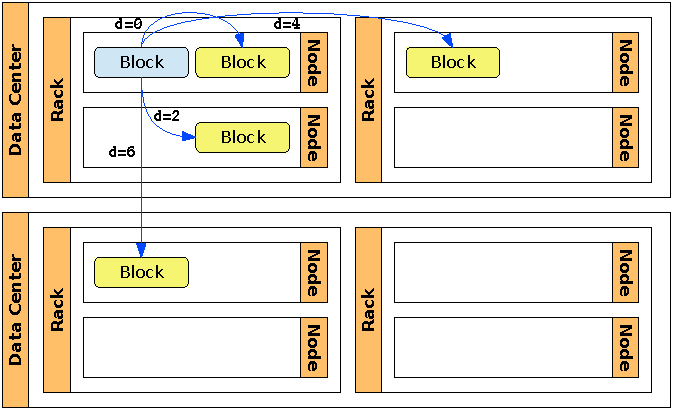
\includegraphics[width=0.75\textwidth]{imagenes/018.pdf}
 \caption{Ejemplo de valores de distancias internodales}
\label{fig:distnodos}
\end{center}
\end{figure}



\subsubsection{Replicaci\'on}\label{subsubsec:replicacionbloques}
\noindent La replicaci\'on es una t\'ecnica transparente al usuario y controlada por el NameNode que, para ser explotado en \'optimas condiciones, deber\'ia tener conocimiento de la distancia internodal. El grado de separaci\'on entre dos r\'eplicas es directamente proporcional al grado de robustez que aporta la copia ---la tolerancia a fallo--- e inversamente proporcional a la eficiencia de transmisi\'on por red, puesto que el ancho de banda disponible para mover un bloque entre dos centros de datos, ser\'a menor que para gestionar la r\'eplica de modo local al nodo, como ya hemos indicado. De tal manera que si se produjese la ca\'ida de un computador, la probabilidad de propagaci\'on de esa ca\'ida disminuye a medida que nos alejamos del nodo problem\'atico ---imaginemos una inundaci\'on del centro de datos, por ejemplo.\newline

La estrategia concreta que sigue HDFS consiste en colocar la primera r\'eplica en el mismo nodo que el cliente del sistema de ficheros, si \'este pertenece al cl\'uster de almacenamiento ---una aplicaci\'on cliente corriendo en un nodo del cl\'uster HDFS, por ejemplo. En caso de que el cliente sea externo al cl\'uster, se elige un nodo al azar, teniendo en cuenta su carga computacional ---prio\-ri\-zan\-do los de menor carga. La segunda r\'eplica se coloca fuera del rack en el que se encuentre la primera copia; el rack concreto se elige al azar. La tercera se emplaza en el mismo rack que la segunda copia pero en un nodo diferente, de nuevo eligiendo al azar y balanceando carga. Las r\'eplicas sucesivas ---el factor de replicaci\'on se controla en el fichero de despliegue de HDFS--- se env\'ian a nodos, siempre diferentes, de este \'ultimo rack.\newline

La mec\'anica descrita aporta el equilibrio deseable entre tolerancia a fallo (ya que habr\'a copias de cada bloque en dos racks distintos), ancho de banda consumido (ya que la escritura de cada bloque s\'olo atraviesa un \emph{switch} o enrutador y las copias sucesivas se hacen dentro del mismo rack), rendimiento de lectura (al poder elegir entre dos racks ante cada petici\'on de lectura de un bloque) y distribuci\'on equilibrada de los bloques en el cl\'uster (que realiza HDFS al ejecutar el m\'etodo descrito). La figura \ref{fig:repbloque} muestra un ejemplo de replicaci\'on con factor 3 en un solo centro de datos. El n\'umero entre corchetes indica el orden de creaci\'on de cada copia; el bloque original, recientemente actualizado o creado, es el azul.

\begin{figure}[tbp]
\begin{center}
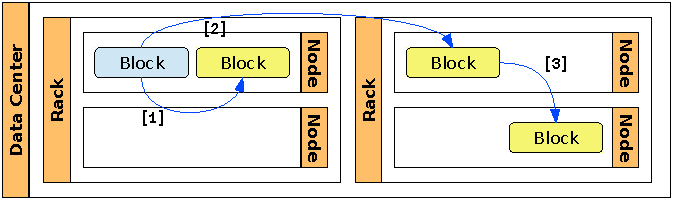
\includegraphics[width=0.75\textwidth]{imagenes/019.pdf}
 \caption{Ejemplo de replicaci\'on de un bloque, factor 3}
\label{fig:repbloque}
\end{center}
\end{figure}


\section{Hadoop MapReduce}\label{sec:hadoopmapred}
\noindent En un cl\'uster t\'ipico sobre HDFS se dispone la capa de operaci\'on de Hadoop, Hadoop MapReduce, que lleva a cabo la ejecuci\'on de los trabajos de mapeo y reducci\'on enviados al framework. Habiendo ya introducido las bases del paradigma MapReduce, corresponde ahora especificar aquellas desviaciones concretas de la implementaci\'on en Hadoop. Como era esperable, Hadoop MapReduce se basa en los principios expuestos en el art\'iculo de Google \cite{googlemapreduce} en cuanto a reparto de tareas y gesti\'on de fallos. Su arquitectura de alto nivel no dista mucho de la observada en la capa HDFS y as\'i se distinguen los roles \emph{maestro} y \emph{esclavo}.\newline

Por una parte, aparece el \emph{JobTracker}, encargado de planificar el reparto de las tareas a los nodos del cl\'uster; por la otra, el \emph{TaskTracker}, que ejecuta las tareas en los nodos como funciones Map y Reduce.\newline

Igual que su sistema de ficheros distribuido, Hadoop MapReduce est\'a escrito en Java.


\subsection{Roles de los nodos}\label{subsec:rolesnodosmapred}
\noindent La figura \ref{fig:desplieguehadoopmapred} representa un despliegue t\'ipico de Hadoop MapReduce en un cl\'uster, utilizando HDFS como sistema de ficheros distribuido soporte. Para completar la \emph{fotograf\'ia} habr\'ia que incluir los nodos responsables de gestionar el HDFS ---NameNode, Checkpoint Node y Backup Node--- omitidos por claridad.

\begin{figure}[tbp]
\begin{center}
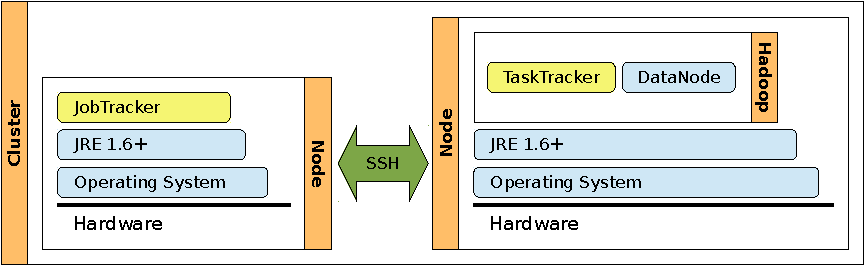
\includegraphics[width=0.99\textwidth]{imagenes/020.pdf}
 \caption{Ejemplo de despliegue de Hadoop MapReduce}
\label{fig:desplieguehadoopmapred}
\end{center}
\end{figure}

\subsubsection{JobTracker}\label{subsubsec:jobtracker}
\noindent El comportamiento del nodo JobTracker es muy similar al expuesto en el caso del NameNode de HDFS, pero aplicado a la gesti\'on de trabajos y tareas. Ante una petici\'on de ejecuci\'on, el JobTracker dividir\'a el trabajo asociado en tareas que repartir\'a entre los TaskTrackers que tenga bajo supervisi\'on. Normalmente, el tama\~no de los ficheros de entrada de las tareas se hace coincidir con el de los bloques del sistema de ficheros distribuido, sea o no HDFS, por ser lo m\'as eficaz. Para cerciorarse de que las ejecuciones concluyen con \'exito en un entorno expuesto al fallo, el JobTracker mantiene una lista de estado de las tareas asociadas a los nodos TaskTracker. De tal forma, en caso de que se produjese un error que impidiese la finalizaci\'on de alguna tarea, ya sea una tarea Map o una Reduce, el JobTracker replanificar\'ia su ejecuci\'on en otro nodo disponible con la m\'inima carga computacional.\newline

El reparto de trabajo se lleva a cabo siguiendo la m\'axima localidad, esto es, haciendo que los TaskTrackers reduzcan tareas basadas en la transformaci\'on de datos almacenados en el mismo nodo. As\'i se reducen tanto el tiempo de acceso al dato del TaskTracker, como la saturaci\'on de la red del cl\'uster, haciendo la computaci\'on m\'as ligera.\newline

Tal y como suced\'ia en la definici\'on general del MapReduce de Google \cite{googlemapreduce}, el fallo en un JobTracker es muy problem\'atico porque s\'olo est\'a cubierta la posibilidad de correr uno por cl\'uster sin usar herramientas adicionales. Dada una ca\'ida en el JobTracker, el procedimiento de recuperaci\'on ``resuelve'' la situaci\'on descartando los trabajos sin concluir; esperando que el nuevo JobTracker pueda hacerse cargo del procesado de esos trabajos incompletos que habr\'an de ser enviados manualmente por los usuarios. Actualmente s\'i se pueden manejar JobTrackers adicionales en un mismo cl\'uster e instante temporal usando una herramienta adicional: \emph{Zookeeper}.


\subsubsection{TaskTracker}\label{subsubsec:tasktracker}
\noindent La misi\'on fundamental del TaskTracker es procesar las tareas que le sean enviadas desde el JobTracker. Peri\'odicamente, el TaskTracker env\'ia una se\~nal a su JobTracker para informar acerca del estado de progreso de la ejecuci\'on de una tarea, si tuviese una asignada, o para indicar que se encuentra a la espera. Si el JobTracker no recibiese esa se\~nal en un intervalo convenido, \'este marcar\'ia el TaskTracker y \emph{todas} sus tareas relacionadas ---las concluidas y las incompletas--- como inaccesibles. Esta clase de fallo, es decir la ca\'ida de un TaskTracker, se considera menos problem\'atico que en el caso del JobTracker, pero implica replanificaci\'on de tareas e incluso repetici\'on de la ejecuci\'on de alguna. Usando la comentada lista de estado de las tareas, el JobTracker buscar\'a las inaccesibles necesarias ---las Map completadas y las Reduce cuya salida no est\'e en el DFS--- y har\'a la redistribuci\'on siguiendo la mec\'anica descrita.
